\documentclass[11pt]{article}
\usepackage[utf8]{inputenc}
\usepackage[a4paper, bottom=65pt, top=65pt, left=60pt, right=60pt]{geometry}
\usepackage[round]{natbib}
\usepackage{booktabs}
\usepackage{float}
\usepackage{amsmath}
\usepackage{subcaption}
\usepackage{graphicx}
\usepackage{microtype}
\usepackage{longtable}
\usepackage[font=small]{caption}


\makeatletter
\renewcommand\maketitle
  {\noindent
   {\Large\bfseries\@title}%
   \medskip\par\noindent
   {\large\bfseries\@author}%
   \hfill
   {\large\@date}%
   \bigskip\par\noindent
  }
\makeatother


\setlength{\parindent}{0pt}

\title{Machine Learning 441 Assignment 1}
\author{David Nicolay (26296918)}
\date{14 August 2025}

\begin{document}


\maketitle
\endgraf\rule{\textwidth}{.8pt}

\section*{Task 1: Analytics Base Table}
\begin{enumerate}
	\item 581012
	\item 62
	\item Fo continuous features see Table~\ref{tab:cts_quality}. For categorical features see Table~\ref{tab:categorical_quality}.
\begin{table}[ht]
	\centering
	\caption{Data Quality Report for Continuous Features}
	\label{tab:cts_quality}
	
		\resizebox{\textwidth}{!}{%
	\begin{tabular}{|l|r|r|r|r|r|r|r|r|r|r|}
		\hline
		\textbf{Feature} & \textbf{Count} & \textbf{\% Miss.} & \textbf{Card.} & \textbf{Min.} & \textbf{$1^{st}$ Qrt.} & \textbf{Mean} & \textbf{Median} & \textbf{$3^{rd}$ Qrt.} & \textbf{Max.} & \textbf{Std. Dev.} \\
		\hline
		1 & 581012 & 0.00 & 1978 & 2054845.65 & 3104928.15 & 3271134.43 & 3311628.60 & 3496222.05 & 4264440.30 & 309481.13 \\
		2 & 581012 & 0.51 & 361 & 0.00 & 58.00 & 155.66 & 127.00 & 260.00 & 360.00 & 111.91 \\
		3 & 581012 & 0.00 & 576099 & 0.00 & 145.49 & 389.92 & 318.12 & 652.53 & 903.48 & 280.34 \\
		4 & 581012 & 0.05 & 67 & 0.00 & 9.00 & 14.10 & 13.00 & 18.00 & 66.00 & 7.49 \\
		5 & 581012 & 0.51 & 569 & -691.00 & 108.00 & 269.42 & 218.00 & 384.00 & 1397.00 & 212.56 \\
		6 & 581012 & 0.00 & 581012 & -173.07 & 6.99 & 46.42 & 29.91 & 68.97 & 600.95 & 58.30 \\
		7 & 581012 & 0.51 & 577988 & -1.00 & -0.50 & -0.00 & -0.00 & 0.50 & 1.00 & 0.58 \\
		8 & 581012 & 0.00 & 5811 & 0.00 & 1106.00 & 8158.11 & 1997.00 & 3328.00 & 510165098.00 & 1185156.02 \\
		9 & 581012 & 0.51 & 207 & 0.00 & 198.00 & 212.14 & 218.00 & 231.00 & 254.00 & 26.77 \\
		11 & 581012 & 0.00 & 255 & 0.00 & 119.00 & 142.53 & 143.00 & 168.00 & 254.00 & 38.27 \\
		12 & 581012 & 0.51 & 5826 & 0.00 & 1024.00 & 1980.43 & 1710.00 & 2550.00 & 7173.00 & 1324.25 \\
		61 & 581012 & 0.00 & 581012 & 1.00 & 145253.75 & 290506.50 & 290506.50 & 435759.25 & 581012.00 & 167723.86 \\
		\hline
	\end{tabular}
}
\end{table}

\begin{table}[H]
	\caption{Categorical Data Quality Report}
	\label{tab:categorical_quality}
	\resizebox{\textwidth}{!}{%
	\begin{tabular}{|l|r|r|r|l|r|r|l|r|r|}
		\hline
		\textbf{Feature} & \textbf{Count} & \textbf{\%miss }& \textbf{Card.} & \textbf{Mode} & \textbf{Mode Freq.} & \textbf{Mode \%} & \textbf{$2^{nd}$ Mode} & \textbf{$2^{nd}$ Mode Freq} & \textbf{$2^{nd}$ Mode \%} \\
		\hline
		10 & 578069 & 0.51 & 186 & 231 & 13482 & 2.33 & 228 & 13474 & 2.33 \\
		13 & 578069 & 0.51 & 2 & 0.00 & 318579 & 55.11 & 1.00 & 259490 & 44.89 \\
		14 & 581012 & 0.00 & 2 & 0 & 551128 & 94.86 & 1 & 29884 & 5.14 \\
		15 & 581012 & 0.00 & 2 & 0 & 327648 & 56.39 & 1 & 253364 & 43.61 \\
		16 & 578069 & 0.51 & 1 & 0.00 & 578069 & 100.00 &  & 0 & 0.00 \\
		17 & 581012 & 0.00 & 1 & 0 & 581012 & 100.00 &  & 0 & 0.00 \\
		18 & 578069 & 0.51 & 3 & 0.00 & 538608 & 93.17 & 1.00 & 36589 & 6.33 \\
		19 & 581012 & 0.00 & 2 & 0 & 291278 & 50.13 & 1 & 289734 & 49.87 \\
		20 & 577566 & 0.59 & 2 & 0.00 & 574553 & 99.48 & 1.00 & 3013 & 0.52 \\
		21 & 173355 & 70.16 & 2 & 0.00 & 172455 & 99.48 & 1.00 & 900 & 0.52 \\
		22 & 581012 & 0.00 & 2 & 0 & 573487 & 98.70 & 1 & 7525 & 1.30 \\
		23 & 581012 & 0.00 & 2 & 0 & 576189 & 99.17 & 1 & 4823 & 0.83 \\
		24 & 581012 & 0.00 & 2 & 0 & 568616 & 97.87 & 1 & 12396 & 2.13 \\
		25 & 581012 & 0.00 & 2 & 0 & 579415 & 99.73 & 1 & 1597 & 0.27 \\
		26 & 581012 & 0.00 & 2 & 0 & 574437 & 98.87 & 1 & 6575 & 1.13 \\
		27 & 581012 & 0.00 & 2 & 0 & 580907 & 99.98 & 1 & 105 & 0.02 \\
		28 & 581012 & 0.00 & 2 & 0 & 580833 & 99.97 & 1 & 179 & 0.03 \\
		29 & 581012 & 0.00 & 2 & 0 & 579865 & 99.80 & 1 & 1147 & 0.20 \\
		30 & 581012 & 0.00 & 2 & 0 & 548378 & 94.38 & 1 & 32634 & 5.62 \\
		31 & 581012 & 0.00 & 2 & 0 & 568602 & 97.86 & 1 & 12410 & 2.14 \\
		32 & 581012 & 0.00 & 2 & 0 & 551041 & 94.84 & 1 & 29971 & 5.16 \\
		33 & 581012 & 0.00 & 2 & 0 & 563581 & 97.00 & 1 & 17431 & 3.00 \\
		34 & 581012 & 0.00 & 2 & 0 & 580413 & 99.90 & 1 & 599 & 0.10 \\
		35 & 581012 & 0.00 & 2 & 0 & 581009 & 100.00 & 1 & 3 & 0.00 \\
		36 & 581012 & 0.00 & 2 & 0 & 578167 & 99.51 & 1 & 2845 & 0.49 \\
		37 & 581012 & 0.00 & 2 & 0 & 577590 & 99.41 & 1 & 3422 & 0.59 \\
		38 & 581012 & 0.00 & 2 & 0 & 579113 & 99.67 & 1 & 1899 & 0.33 \\
		39 & 581012 & 0.00 & 2 & 0 & 576991 & 99.31 & 1 & 4021 & 0.69 \\
		40 & 581012 & 0.00 & 2 & 0 & 571753 & 98.41 & 1 & 9259 & 1.59 \\
		41 & 581012 & 0.00 & 2 & 0 & 580174 & 99.86 & 1 & 838 & 0.14 \\
		42 & 581012 & 0.00 & 2 & 0 & 547639 & 94.26 & 1 & 33373 & 5.74 \\
		43 & 581012 & 0.00 & 2 & 0 & 523260 & 90.06 & 1 & 57752 & 9.94 \\
		44 & 581012 & 0.00 & 2 & 0 & 559734 & 96.34 & 1 & 21278 & 3.66 \\
		45 & 581012 & 0.00 & 2 & 0 & 580538 & 99.92 & 1 & 474 & 0.08 \\
		46 & 581012 & 0.00 & 2 & 0 & 578423 & 99.55 & 1 & 2589 & 0.45 \\
		47 & 581012 & 0.00 & 2 & 0 & 579926 & 99.81 & 1 & 1086 & 0.19 \\
		48 & 581012 & 0.00 & 2 & 0 & 580066 & 99.84 & 1 & 946 & 0.16 \\
		49 & 581012 & 0.00 & 2 & 0 & 465765 & 80.16 & 1 & 115247 & 19.84 \\
		50 & 581012 & 0.00 & 2 & 0 & 550842 & 94.81 & 1 & 30170 & 5.19 \\
		51 & 581012 & 0.00 & 2 & 0 & 555346 & 95.58 & 1 & 25666 & 4.42 \\
		52 & 581012 & 0.00 & 2 & 0 & 528493 & 90.96 & 1 & 52519 & 9.04 \\
		53 & 581012 & 0.00 & 2 & 0 & 535858 & 92.23 & 1 & 45154 & 7.77 \\
		54 & 581012 & 0.00 & 2 & 0 & 579401 & 99.72 & 1 & 1611 & 0.28 \\
		55 & 581012 & 0.00 & 2 & 0 & 579121 & 99.67 & 1 & 1891 & 0.33 \\
		56 & 581012 & 0.00 & 2 & 0 & 580893 & 99.98 & 1 & 119 & 0.02 \\
		57 & 581012 & 0.00 & 2 & 0 & 580714 & 99.95 & 1 & 298 & 0.05 \\
		58 & 581012 & 0.00 & 2 & 0 & 565439 & 97.32 & 1 & 15573 & 2.68 \\
		59 & 581012 & 0.00 & 2 & 0 & 567206 & 97.62 & 1 & 13806 & 2.38 \\
		60 & 581012 & 0.00 & 2 & 0 & 572262 & 98.49 & 1 & 8750 & 1.51 \\
		62 & 581012 & 0.00 & 1 & 1 & 581012 & 100.00 &  & 0 & 0.00 \\
		\hline
	\end{tabular}
}

\end{table}


	\item Target feature data quality report:
	\begin{table}[H]
		\caption{Data Quality Report for target feature}
		\label{tab:data_quality}
			\resizebox{\textwidth}{!}{%
		\begin{tabular}{|l|r|r|r|r|r|r|r|r|r|r|}
			\hline
			\textbf{Feature} & \textbf{Count} & \textbf{\%miss }& \textbf{Card.} & \textbf{Mode} & \textbf{Mode Freq.} & \textbf{Mode \%} & \textbf{$2^{nd}$ Mode} & \textbf{$2^{nd}$ Mode Freq} & \textbf{$2^{nd}$ Mode \%}  \\
			\hline
			$T$ & 581012 & 0.01 & 7 & 2.00 & 283269 & 48.75 & 1.00 & 211815 & 36.46\\
			\hline
		\end{tabular}
	}
	\end{table}

\end{enumerate}


\section*{Task 2: Data Quality Issues}
\begin{longtable}{|p{1.7cm}|p{4cm}|p{8cm}|}
	\caption{Feature Quality Issues} \label{tab:feature_quality_issues} \\
	\hline
	\textbf{Feature} & \textbf{Data Quality Issue} & \textbf{Justification} \\
	\hline
	\endfirsthead
	
	\multicolumn{3}{c}%
	{{\bfseries \tablename\ \thetable{} -- continued from previous page}} \\
	\hline
	\textbf{Feature} & \textbf{Data Quality Issue} & \textbf{Justification} \\
	\hline
	\endhead
	
	\hline \multicolumn{3}{|r|}{{Continued on next page}} \\ \hline
	\endfoot
	
	\hline 
	\endlastfoot
	A1, A4, A6, A9, A11, A12 & Outlier observations & It can be observed in Figure~\ref{fig:outliers} that there are outliers present in these features. These boxplots were generated by first standardising the features the using the Interquartile Range (IQR) method to determine an outlier threshold. The IQR method determines the upper bound by calculating $Q3 + 1.5 \times IQR$ and the lower bound using $Q1 - 1.5 \times IQR$. Where $Q$1 is the 25th percentile (first quartile), $Q3$ is the 75th percentile (third quartile), and $IQR = Q3 - Q1$.\\
	\hline
	A2 & Missing values & Many records have missing values for A2 as observed in Table~\ref{tab:cts_quality}. There are 0.51\% of the observations with A2 missing. \\
	\hline
	A2, A3 & Perfect correlation & The features A2 and A3 are perfectly correlated as observed in Figure~\ref{fig:heatmap}. This means that they are an \textit{exact} linear transformation of each other.\\
	\hline
	A4, A5, A7, A9, A10, A12, A13, A16, A18, A20, A21 & Missing values & Testing revealed that there are a certain 2947 rows with all these features missing simultaneously. \\
	\hline
	A5 & Outlier observations & Figure~\ref{fig:f5} raises concern surrounding some values of this feature being negative. Testing revealed that there are 26 outlier negative observations, whilst the rest of this feature contains positive values. \\
	\hline
	A8 & Outlier observations & The maximum value of this feature is much higher than the mean and the 3rd quartile, indicating that there may be an error. The extreme nature of these outliers is shown in Figure~\ref{fig:f8}. Through testing it was found that there are 18 observations greater than 50,000,000 with the 99.9th percentile sitting at 6699.0.\\
	\hline
	A9, A11 & Strongly correlated features & Figure~\ref{fig:heatmap} indicates that A9 and A11 are strongly correlated with a coefficient of  -0.78. After further investigation, we observed that there is likely a mathematical or physical constraint between the two features due to the relationship exhibited in Figure~\ref{fig:A9_A11_scatter}.\\
	\hline
	A10 & Abnormal data type & There are 0.99\% of the observations in feature A10 that have the value 'a' whilst all the other observations have numerical values. \\
	\hline
	A14, A18, A30, A32, A42, A43, A50, A52, A53 & Class imbalance, $90\%<$\textit{Mode\%} $< 95\%$ & Table~\ref{tab:categorical_quality} indicates that these features have a class imbalance since their modal class consists of between 90\% and 95\% of the dataset. \\
	\hline
	A16 & Cardinality of 1 & This categorical variable is redundant since all the observations have the same value. This is observed in the cardinality column of Table~\ref{tab:categorical_quality}. \\
	\hline
	A17 & Cardinality of 1 & This categorical variable is redundant since all the observations have the same value. This is observed in the cardinality column of Table~\ref{tab:categorical_quality}. \\
	\hline
	A20, A21, A22, A23, A24, A25, A26, A27, A28, A29, A31, A33, A34, A35, A36, A37, A38, A39, A40, A41, A44, A45, A46, A47, A48, A51, A54, A55, A56, A57, A58, A59, A60 & Severe class imbalance, $95\%\le$\textit{Mode\%} $< 100\%$ & Table~\ref{tab:categorical_quality} indicates that these features have a severe class imbalance since their modal class consists of between 95\% and 100\% of the dataset. \\
	\hline
	A21 & Missing values & Many records, specifically 70.16\%, have missing values for A21 as observed in Table~\ref{tab:categorical_quality}. \\
	\hline
	A35 & Extremely high class imbalance& The 2nd class for this feature only has three observations. This rounds to 0.01\% shown in Table~\ref{tab:categorical_quality}. \\
	\hline
	A61 & ID Feature & This feature has a perfectly uniform distribution observed in Figure~\ref{fig:f61}. Testing revealed that the feature value is exactly the same as the row number for all observations. \\
	\hline
	A61, A1 & Strongly correlated features & The features A1 and A61 are strongly correlated, as observed in Figure~\ref{fig:heatmap} with a correlation coefficient of -0.95. \\
	\hline
	A62 & Cardinality of 1 & This categorical variable is redundant since all the observations have the same value. \\
	\hline
	T & Target class imbalance &  It can be observed in Figure~\ref{fig:target_dist_entire} that there is a severe target class imbalance, with only 2747 observations in class 4.  This means that certain classes are better represented in the dataset and can lead to machine learning model bias. \\
	\hline
	T & Target variable missing values & Testing revealed that there are 60 missing observations in the target variable. This rounds to 0.01\% of the data seen in Table~\ref{tab:data_quality}.\\
	\hline
\end{longtable}

\begin{figure}[H]
	\centering
	
	\begin{minipage}[t]{0.48\textwidth}
		\centering
		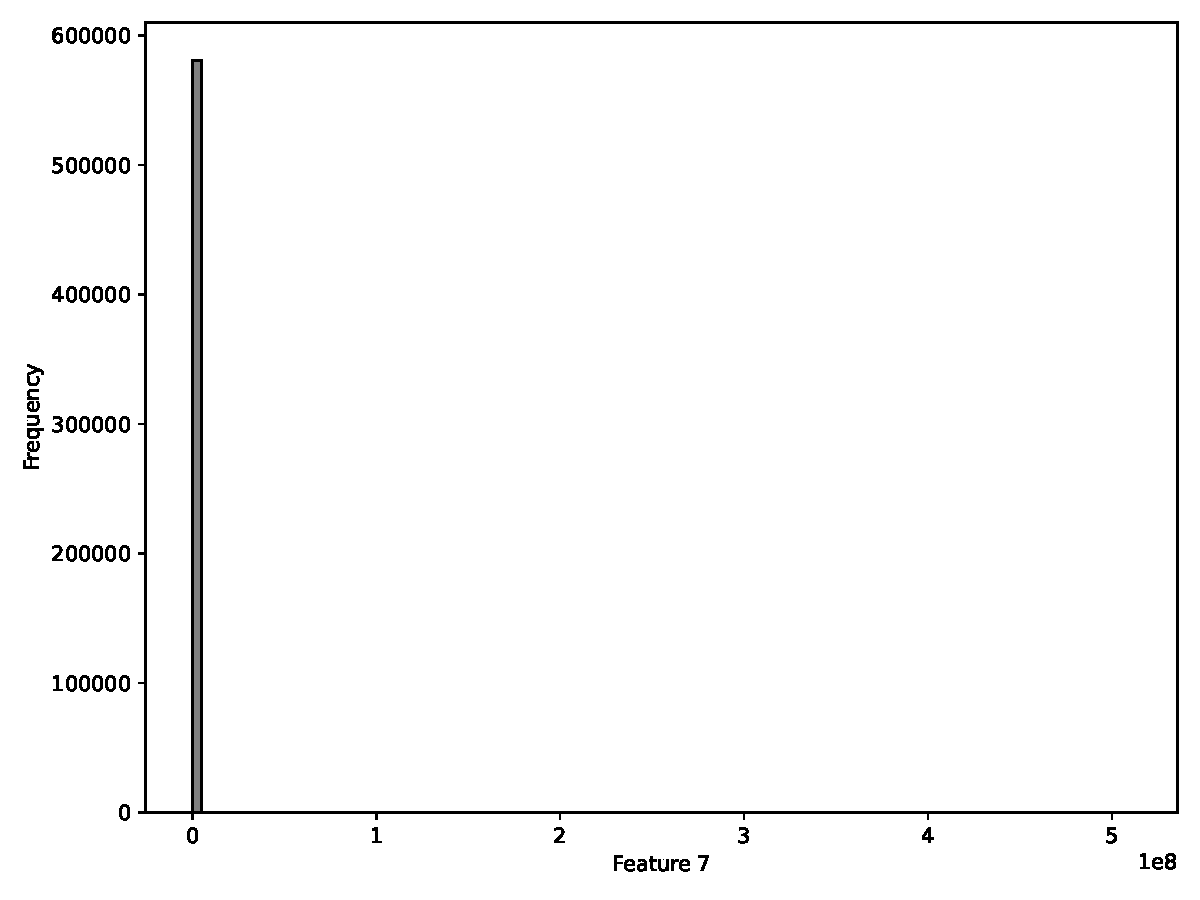
\includegraphics[width=\textwidth]{images/8_distribution.pdf}
		\caption{Feature 8 distribution with 100 bins}
		\label{fig:f8}
	\end{minipage}
	\hfill
	\begin{minipage}[t]{0.48\textwidth}
		\centering
		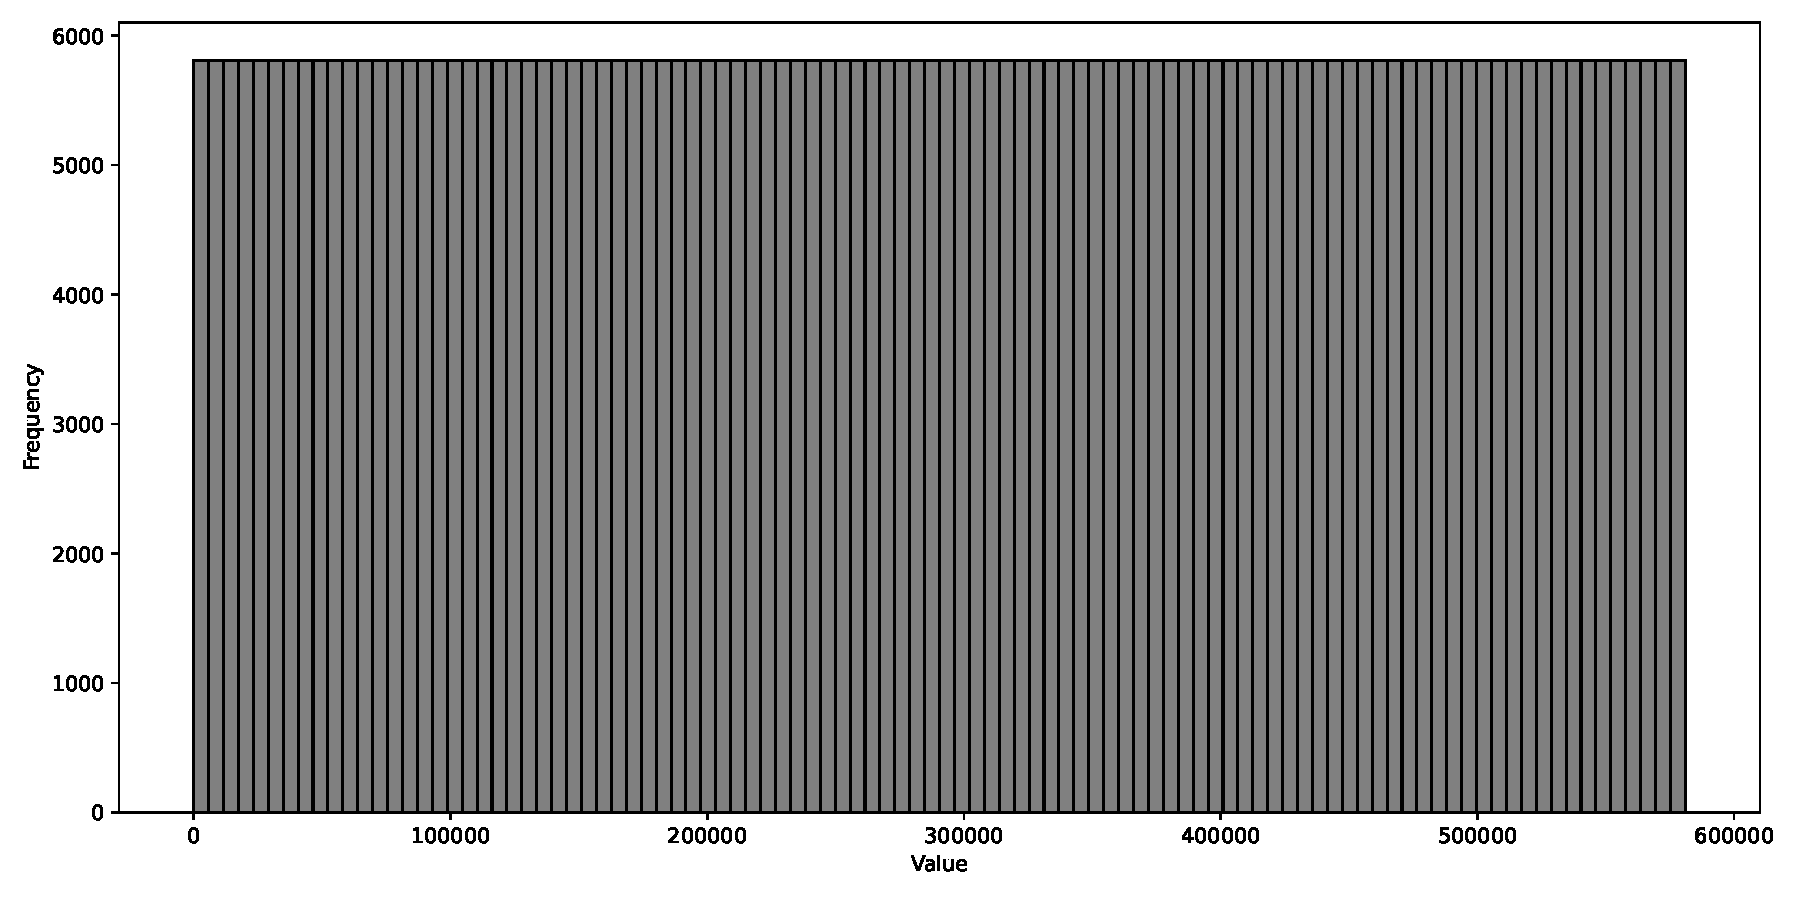
\includegraphics[width=\textwidth]{images/61_distribution.pdf}
		\caption{Feature 61 distribution with 100 bins}
		\label{fig:f61}
	\end{minipage}
	
\end{figure}

\begin{figure}[H]
	\centering
	% Row 1: Feature 2 (left) + Feature 5 (right)
	\begin{minipage}[t]{0.48\textwidth}
		\centering
		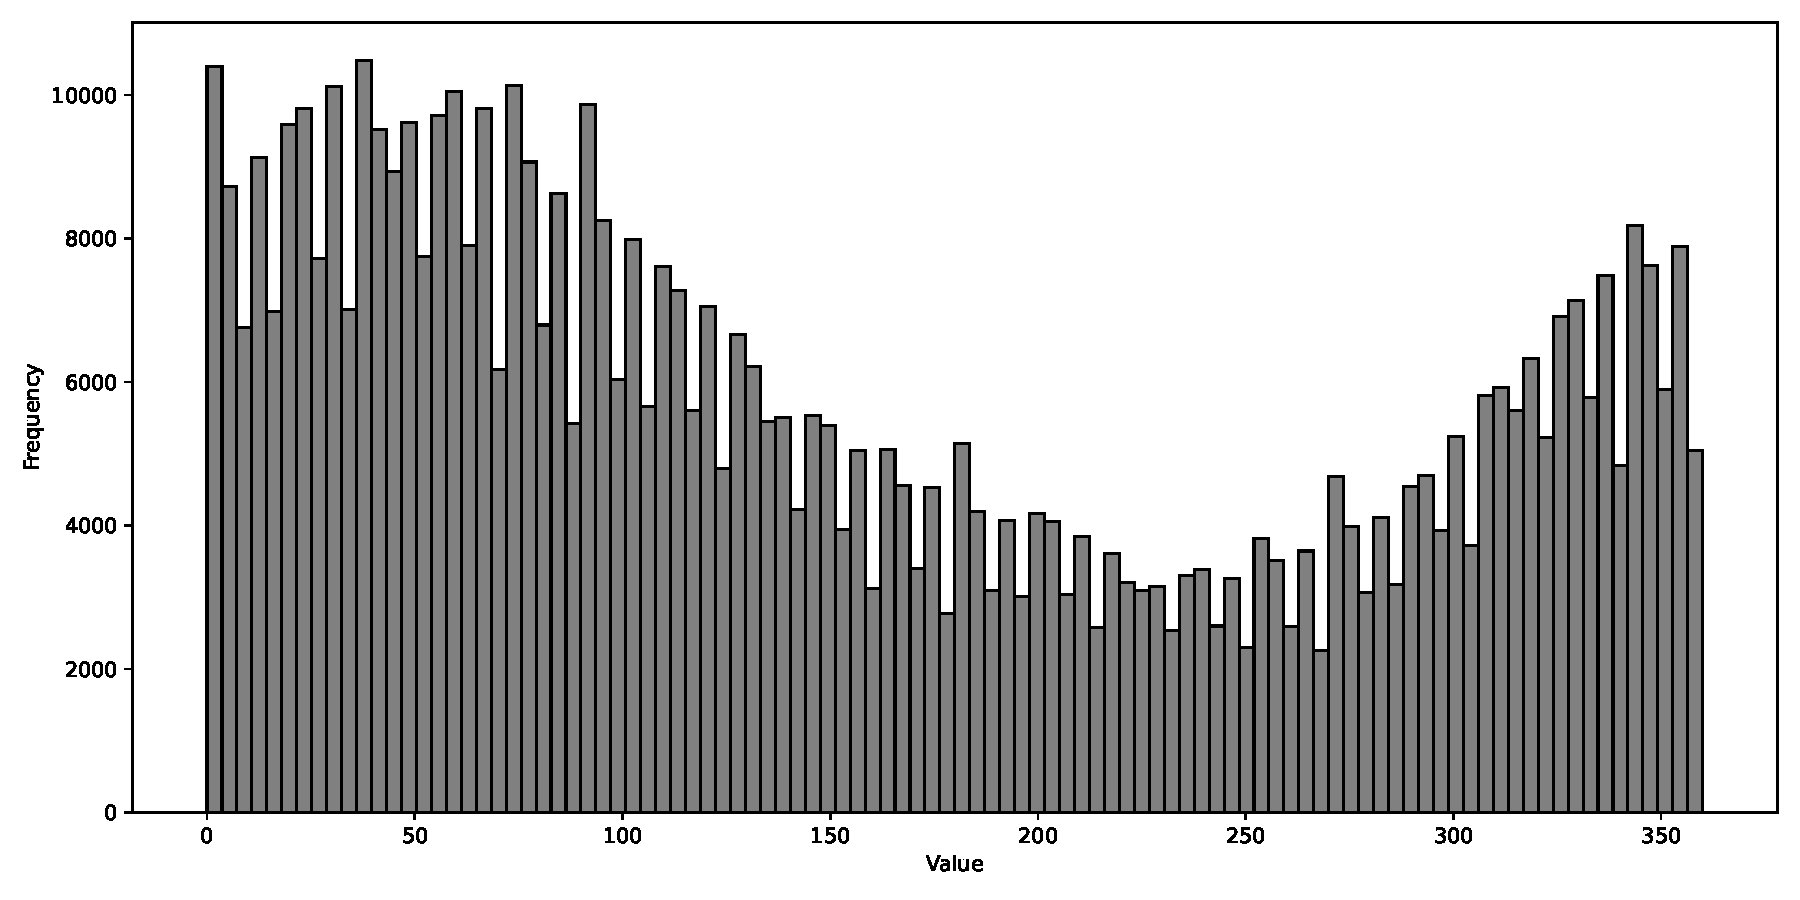
\includegraphics[width=\textwidth]{images/2_distribution.pdf}
		\caption{Feature 2 distribution with 100 bins}
		\label{fig:f2}
	\end{minipage}
	\hfill
	\begin{minipage}[t]{0.48\textwidth}
		\centering
		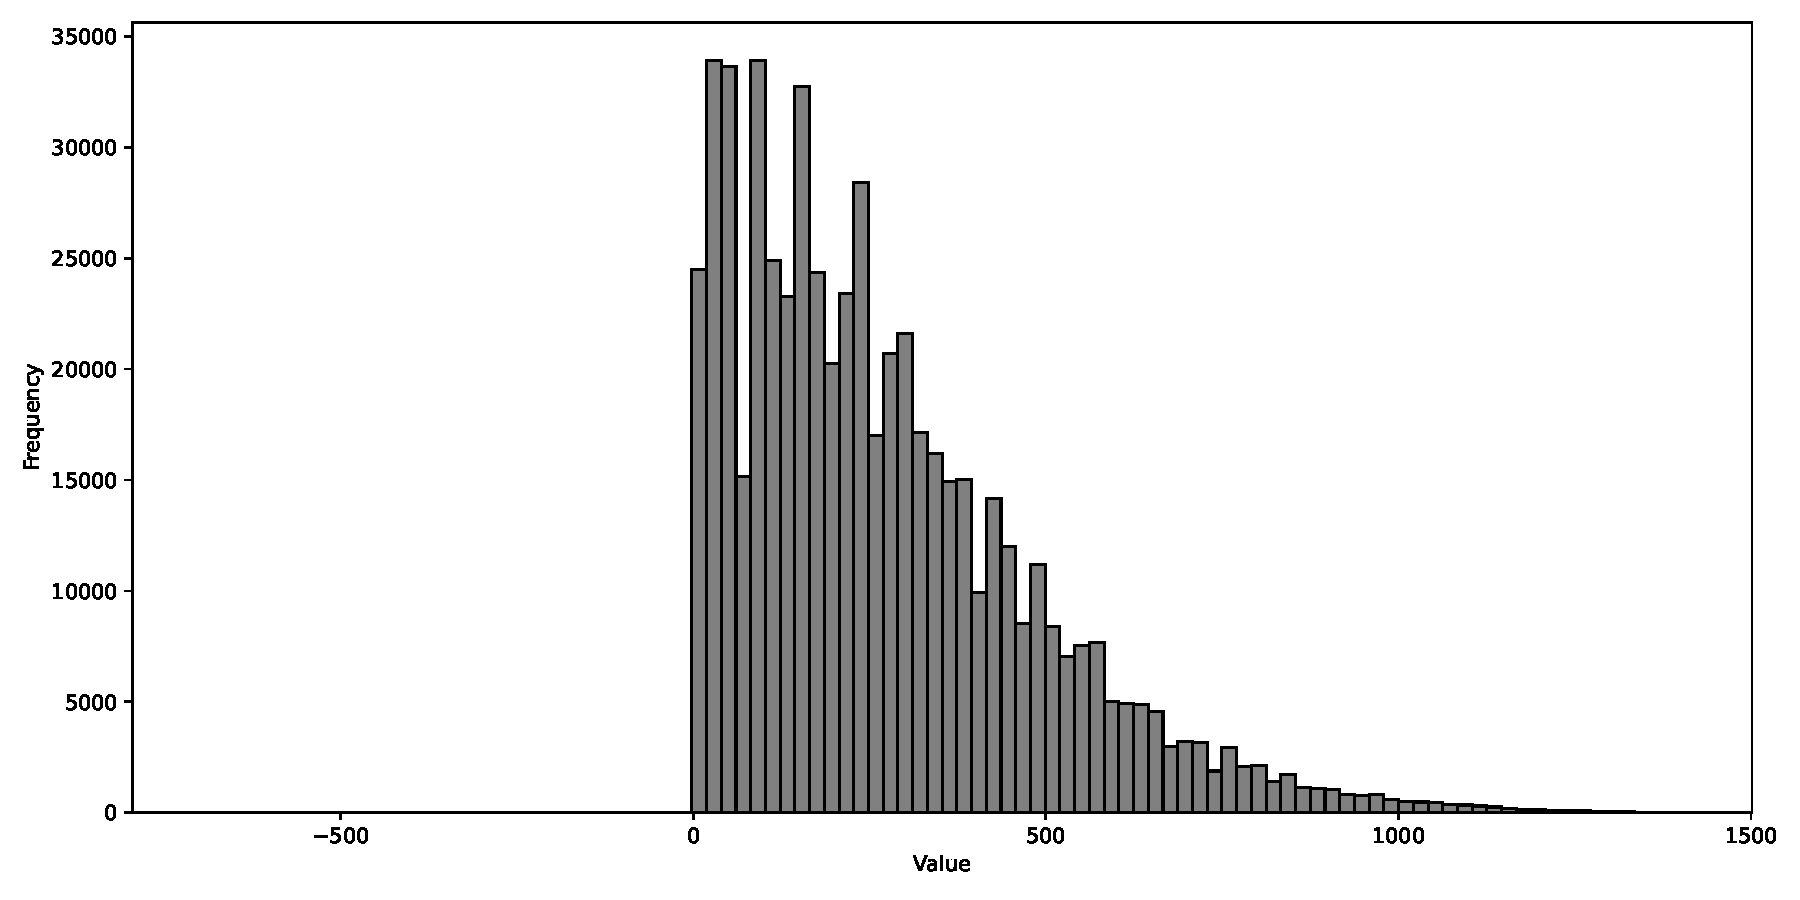
\includegraphics[width=\textwidth]{images/5_distribution.pdf}
		\caption{Feature 5 distribution with 100 bins}
		\label{fig:f5}
	\end{minipage}
	


\end{figure}






\begin{figure}[H]
	\centering
	% First plot (heatmap)
	\begin{minipage}[t]{0.48\textwidth}
		\centering
		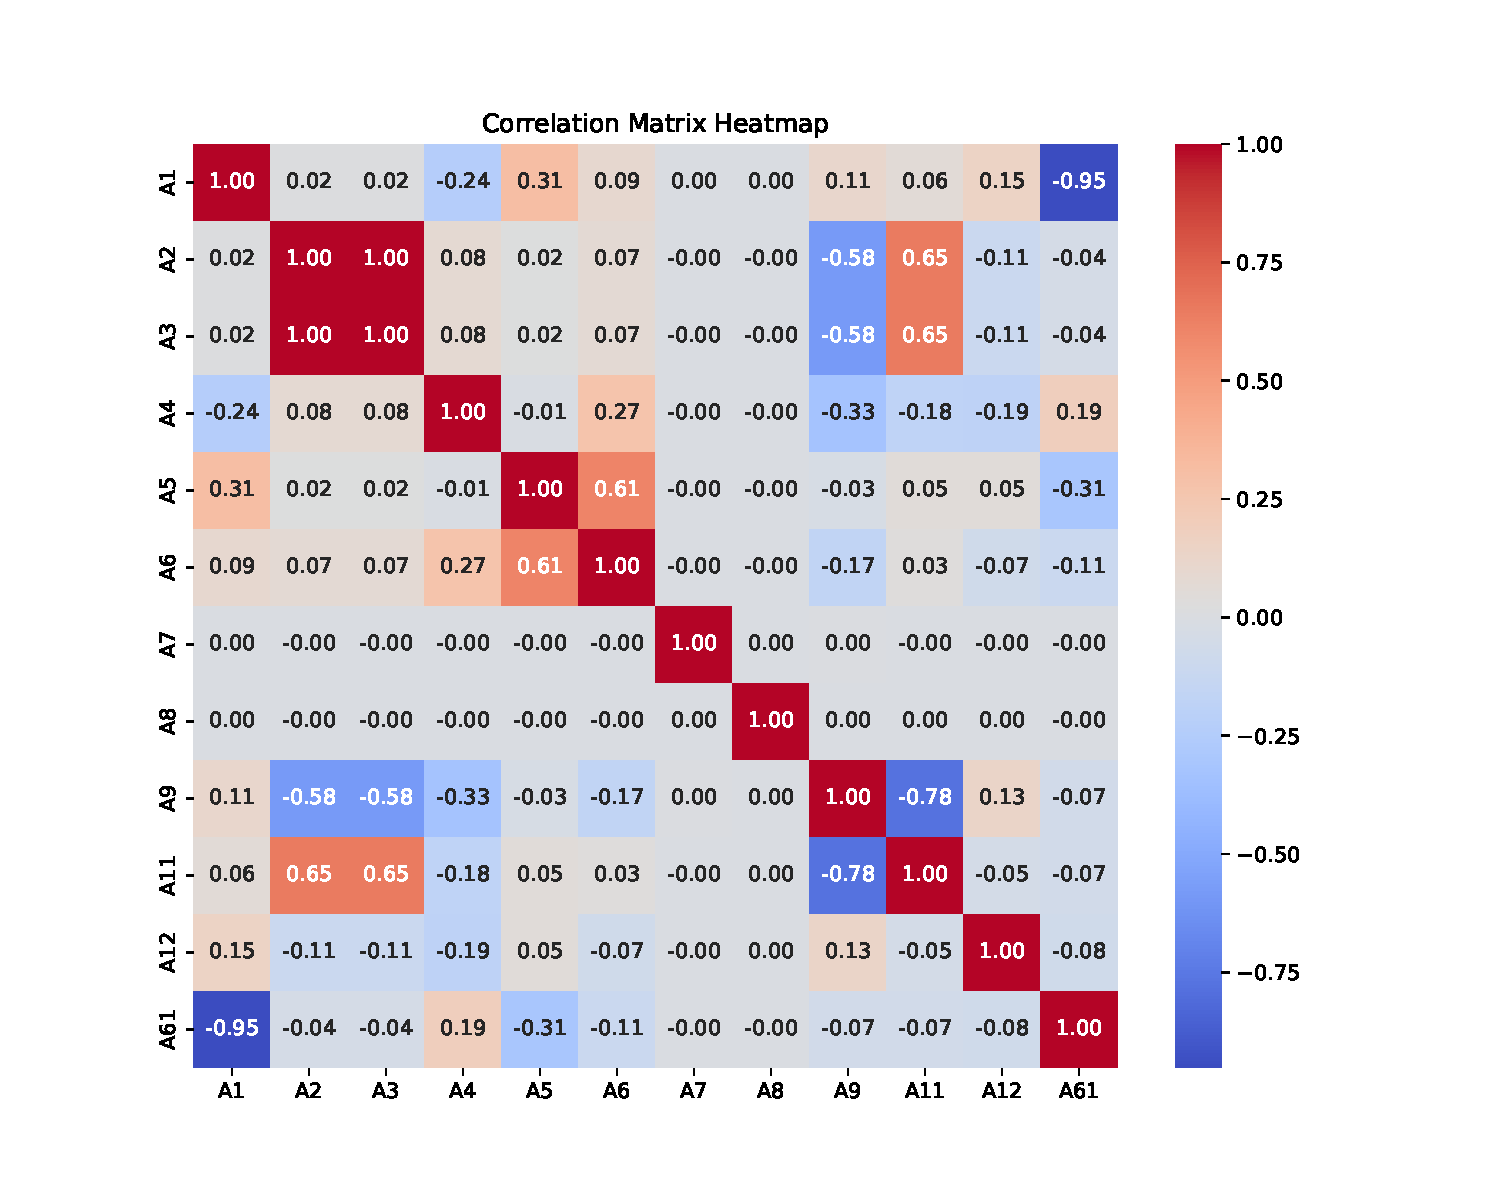
\includegraphics[width=\linewidth]{images/correlation_matrix_heatmap.pdf}
		\caption{Correlation heatmap}
		\label{fig:heatmap}
	\end{minipage}
	\hfill
	% Second plot (scatter)
	\begin{minipage}[t]{0.48\textwidth}
		\centering
		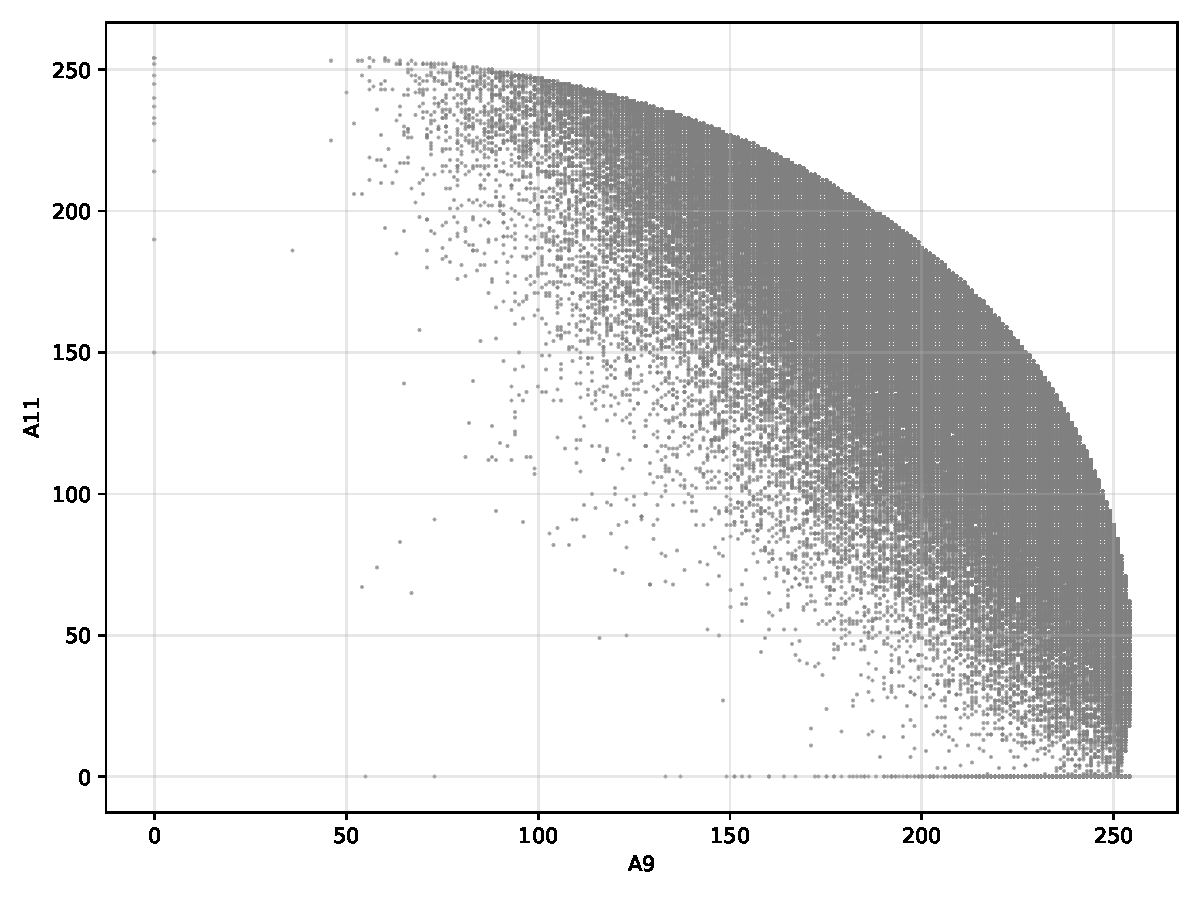
\includegraphics[width=\linewidth]{images/A9_A11_scatter.pdf}
		\caption{A9 vs A11 scatter plot}
		\label{fig:A9_A11_scatter}
	\end{minipage}
\end{figure}

\begin{figure}[H]
	\centering
	\begin{subfigure}[b]{0.48\textwidth}
		\centering
		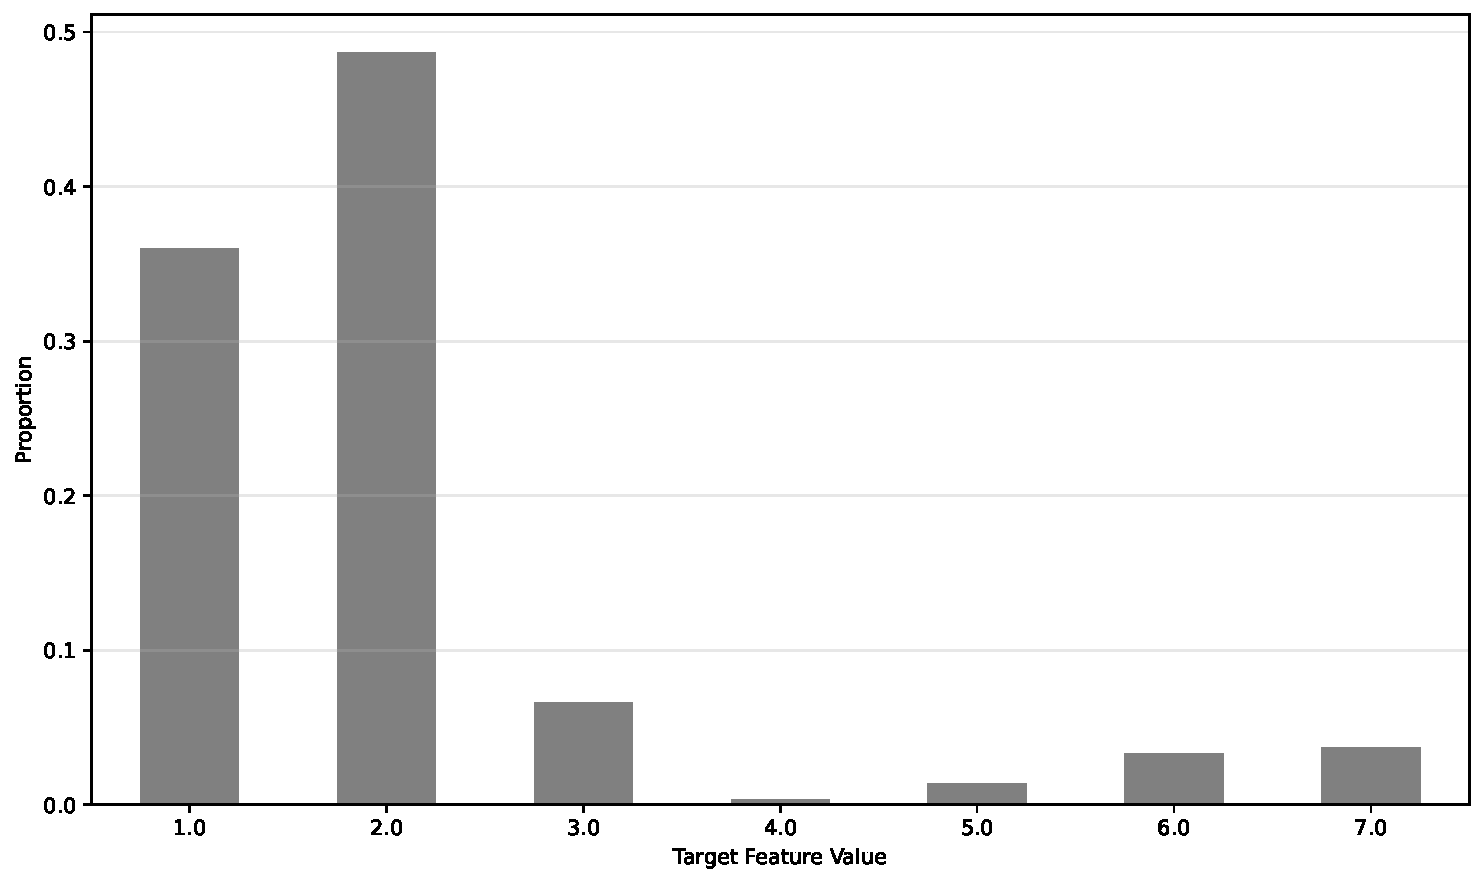
\includegraphics[width=\textwidth]{images/target_feature_distribution_missing.pdf}
		\caption{Target value distribution (missing)}
		\label{fig:target_dist_missing}
	\end{subfigure}
	\hfill
	\begin{subfigure}[b]{0.48\textwidth}
		\centering
		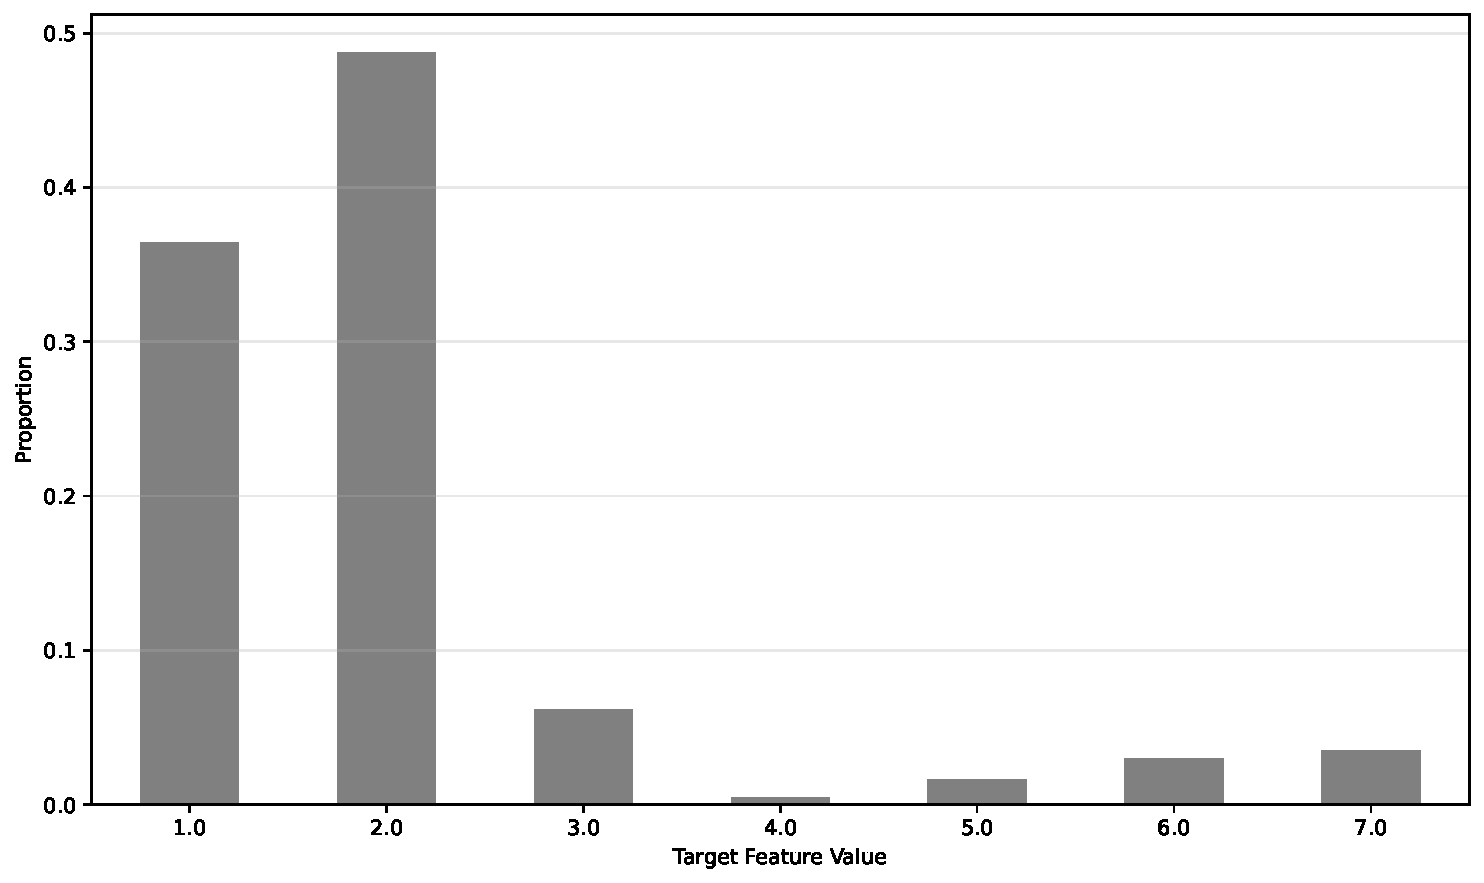
\includegraphics[width=\textwidth]{images/target_feature_distribution_entire.pdf}
		\caption{Target value distribution (entire dataset)}
		\label{fig:target_dist_entire}
	\end{subfigure}
	\caption{Comparison of target value distribution for missing data observations vs entire dataset}
	\label{fig:target_dist}
\end{figure}

\begin{figure}
	\begin{minipage}[t]{\textwidth}
		\centering
		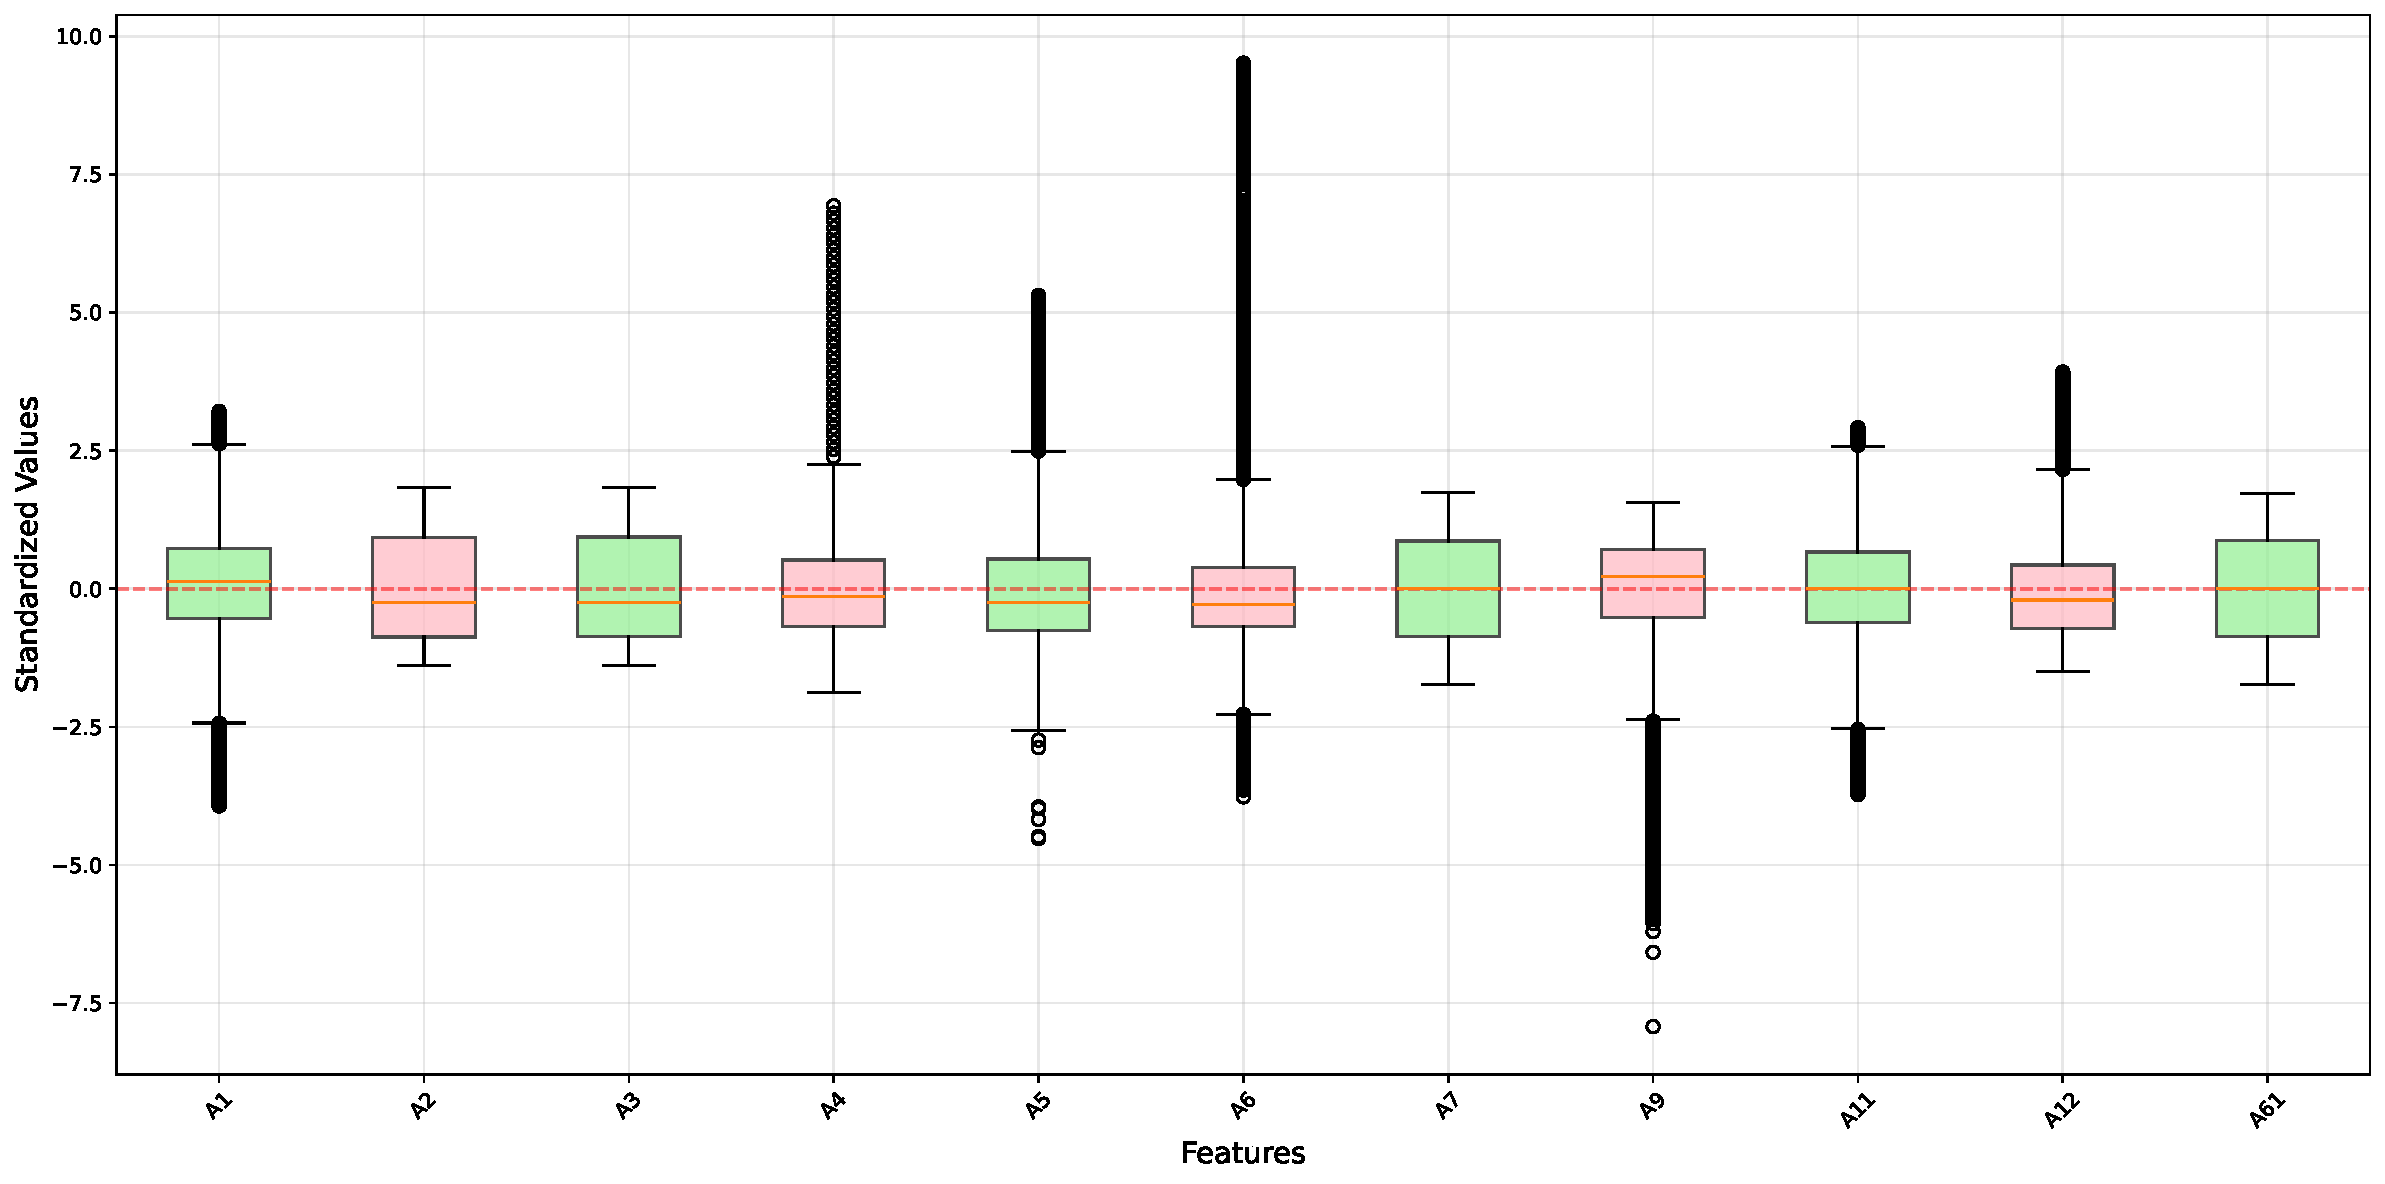
\includegraphics[width=\textwidth]{images/continuous_variables_boxplots_normalized.pdf}
		\caption{Boxplots of standardised continuous variables}
		\label{fig:outliers}
	\end{minipage}
\end{figure}




\section*{Task 3: Addressing The Data Quality Issues}
\begin{longtable}{|p{1.7cm}|p{4cm}|p{3cm}|p{6cm}|}
	\caption{Data Quality Fixes} \label{tab:feature_quality_fixes} \\
	\hline
	\textbf{Feature} & \textbf{Data Quality Issue} & \textbf{Handling Strategy} & \textbf{Justification} \\
	\hline
	\endfirsthead
	
	\multicolumn{4}{c}{{\bfseries \tablename\ \thetable{} -- continued from previous page}} \\
	\hline
	\textbf{Feature} & \textbf{Data Quality Issue} & \textbf{Handling Strategy} & \textbf{Justification} \\
	\hline
	\endhead
	
	\hline \multicolumn{4}{|r|}{{Continued on next page}} \\ \hline
	\endfoot
	
	\hline
	\endlastfoot
	A1, A4, A6, A9, A11, A12 & Outlier observations & Nothing & These outliers can be considered \textit{valid} outliers and should not be removed. This is due to the outliers not appearing to be out of line with the distributions of the feature overall.\\ \hline
	A2 & Missing values & Remove feature & See below. \\ \hline
	A2, A3 & Perfect correlation & Remove feature A2 & Since the features are perfectly correlated, we are essentially storing the same information twice which provides no value to a machine learning model. Since A2 has missing values we might as well remove it to deal with two quality issues at the same time. \\ \hline
	A4, A5, A7, A9, A10, A12, A13, A16, A18, A20, A21 & Missing values & Remove observations & Since testing revealed that there are a certain 2947 rows with all these features missing simultaneously, it makes sense to simply remove all these observations since they have a large amount of missing information. It is useful to note that the distribution of the target variable in these observations matches the overall distribution of the target variable for the whole dataset observed in Figure~\ref{fig:target_dist}. This means that we are not likely to lose any useful information about a certain target category when removing these observations.  \\ \hline
	A5 & Outlier observations & Remove observations & Since there are only 26 negative observations, we can safely drop these as they make up only a minute part of the dataset. \\
	\hline
	A8 & Outlier observations & Remove observations & There must be an error with the observations in question because the outliers are so incredibly skewed. Through testing it was found that there are 18 observations greater than 50,000,000 with the 99.9th percentile sitting at 6699.0. \\ \hline
	A9, A11 & Strongly correlated features & Nothing & Despite these features being strongly correlated, there is still a chance that the features' relationship makes sense in the domain context. Therefore we elect to not remove either feature.\\ \hline
	A10 & Abnormal data type & Remove observations & Testing revealed that the levels of this suspected categorical variable range from 100–254 predominantly. Since many observations have the value 'a', we can guess this error is not at random and the character 'a' could be replaced with 255. This fits the distribution seen in Figure~\ref{fig:f10}. Despite these facts, one would need to consult a domain expert before replacing it by 255, therefore the safer option is to remove the observations. \\ \hline
	A14, A18, A30, A32, A42, A43, A50, A52, A53 & Class imbalance, $90\%<$\textit{Mode\%} $< 95\%$ & Under-sample majority classes & Due to the large number of observations in this dataset, we can safely under-sample the majority class to reduce the class imbalances. If this reduces the dataset's size too much, we can always consider oversampling the minority classes. \\ \hline
	A16 & Cardinality of 1 & Drop feature & This categorical variable can be removed since it will have no effect on a model's performance. \\ \hline
	A17 & Cardinality of 1 & Drop feature & This categorical variable can be removed since it will have no effect on a model's performance. \\ \hline
	A20, A21, A22, A23, A24, A25, A26, A27, A28, A29, A31, A33, A34, A35, A36, A37, A38, A39, A40, A41, A44, A45, A46, A47, A48, A51, A54, A55, A56, A57, A58, A59, A60 & Severe class imbalance, $95\%\le$\textit{Mode\%} $< 100\%$ & Under-sample majority classes & Due to the large number of observations in this dataset, we can safely under-sample the majority class to reduce the class imbalances. If this reduces the dataset's size too much, we can always consider oversampling the minority classes. \\ \hline
	A21 & Missing values & Drop feature & Testing revealed that the correlation between missingness of A21 and the target is -0.0004. This only means that there is not a linear relationship. It is possible that the missingness is still related to the target feature. Plotting the confusion matrix Figure~\ref{fig:a20a21} indicates that A21 has the same values as A20 for every observation. This makes it redundant. Due to the high number of missing values we should remove the feature. It still is worth investigating adding the missingness as an extra category. \\ \hline
	A35 & Extremely high class imbalance & Drop feature & Since there are only three observations in the second class for this feature, it should be removed without affecting model performance. \\ \hline
	A61 & ID Feature & Drop feature & It was confirmed that this feature perfectly fits the description of an ID column, meaning it has no predictive power and can be removed. \\ \hline
	A61, A1 & Strongly correlated features & Drop feature & Since we have already established that A61 is a redundant ID feature and have determined to remove it, we have solved the issue. \\ \hline
	A62 & Cardinality of 1 & Drop feature & This categorical variable can be removed since it will have no effect on a model's performance. \\ \hline
	T & Target class imbalance & Synthetic minority oversampling technique & Since we have so few observations for classes 3, 4, 5, 6 and 7; using SMOTE will help resolve our issue by creating new instances to balance out the classes.  \\ \hline
	T & Target variable missing values & Remove observations & Since such an insignificant number of observations are missing, we can safely drop these observations without affecting the size of our dataset much as all. \\ \hline
\end{longtable}

\begin{figure}
		\begin{minipage}[t]{\textwidth}
		\centering
		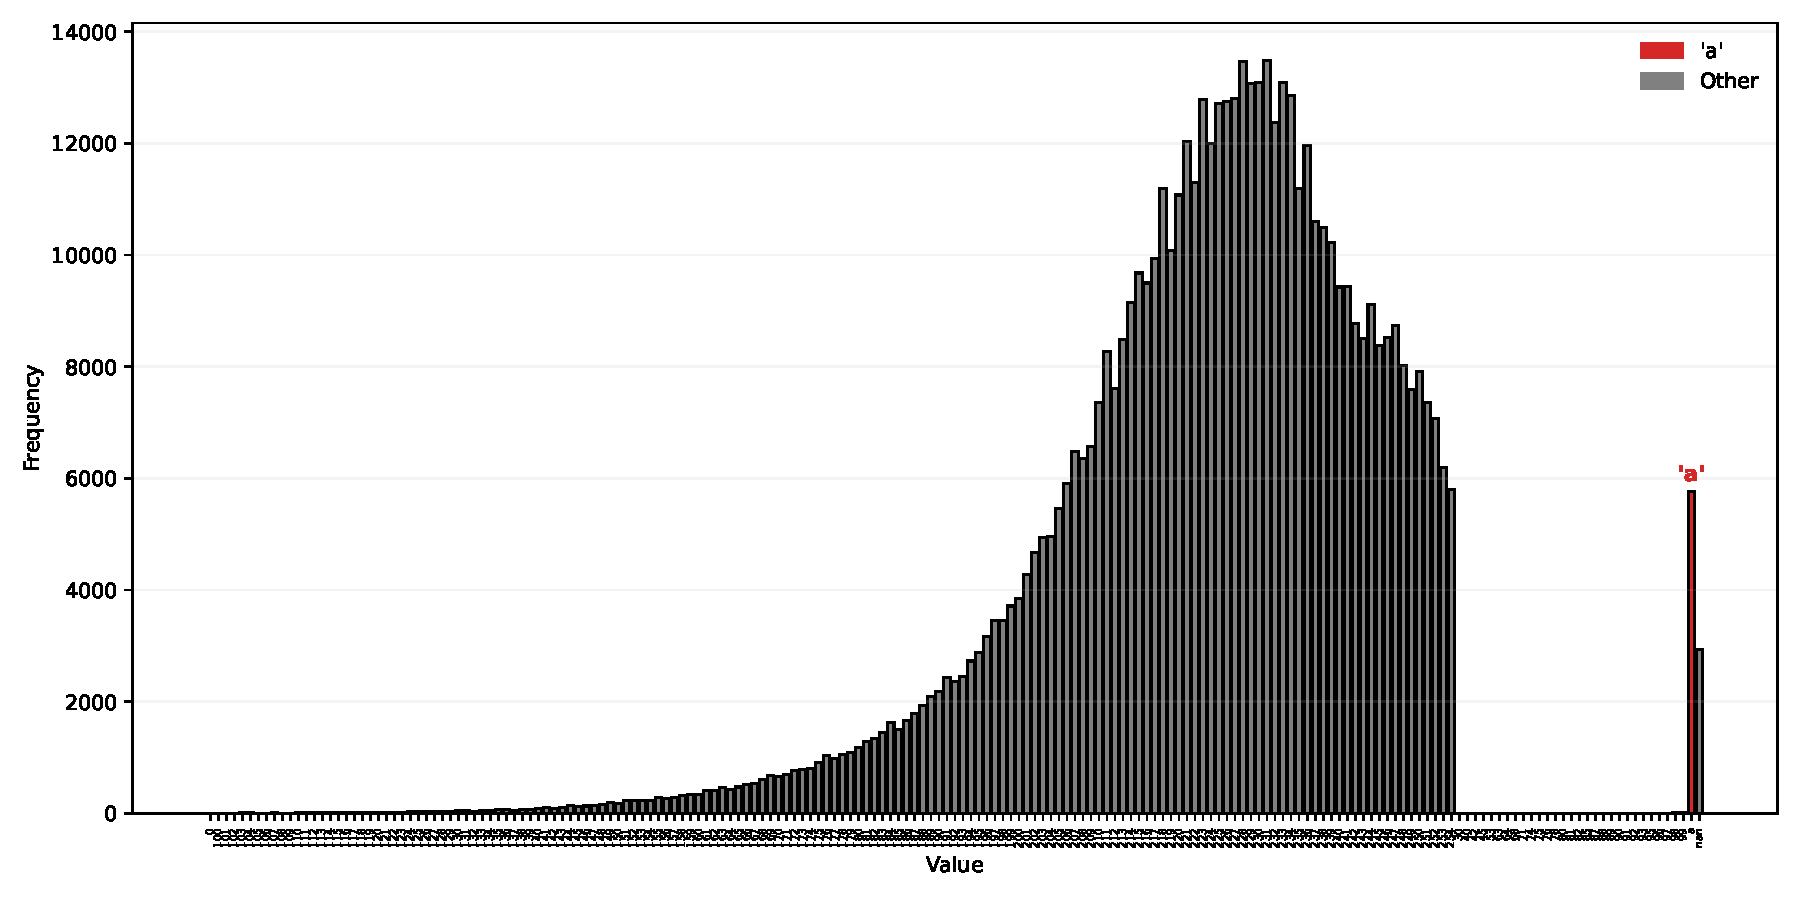
\includegraphics[width=\textwidth]{images/10_distribution.pdf}
		\caption{Feature 10 distribution ordered by value}
		\label{fig:f10}
	\end{minipage}
\end{figure}

\begin{figure}
	\begin{minipage}[t]{\textwidth}
		\centering
		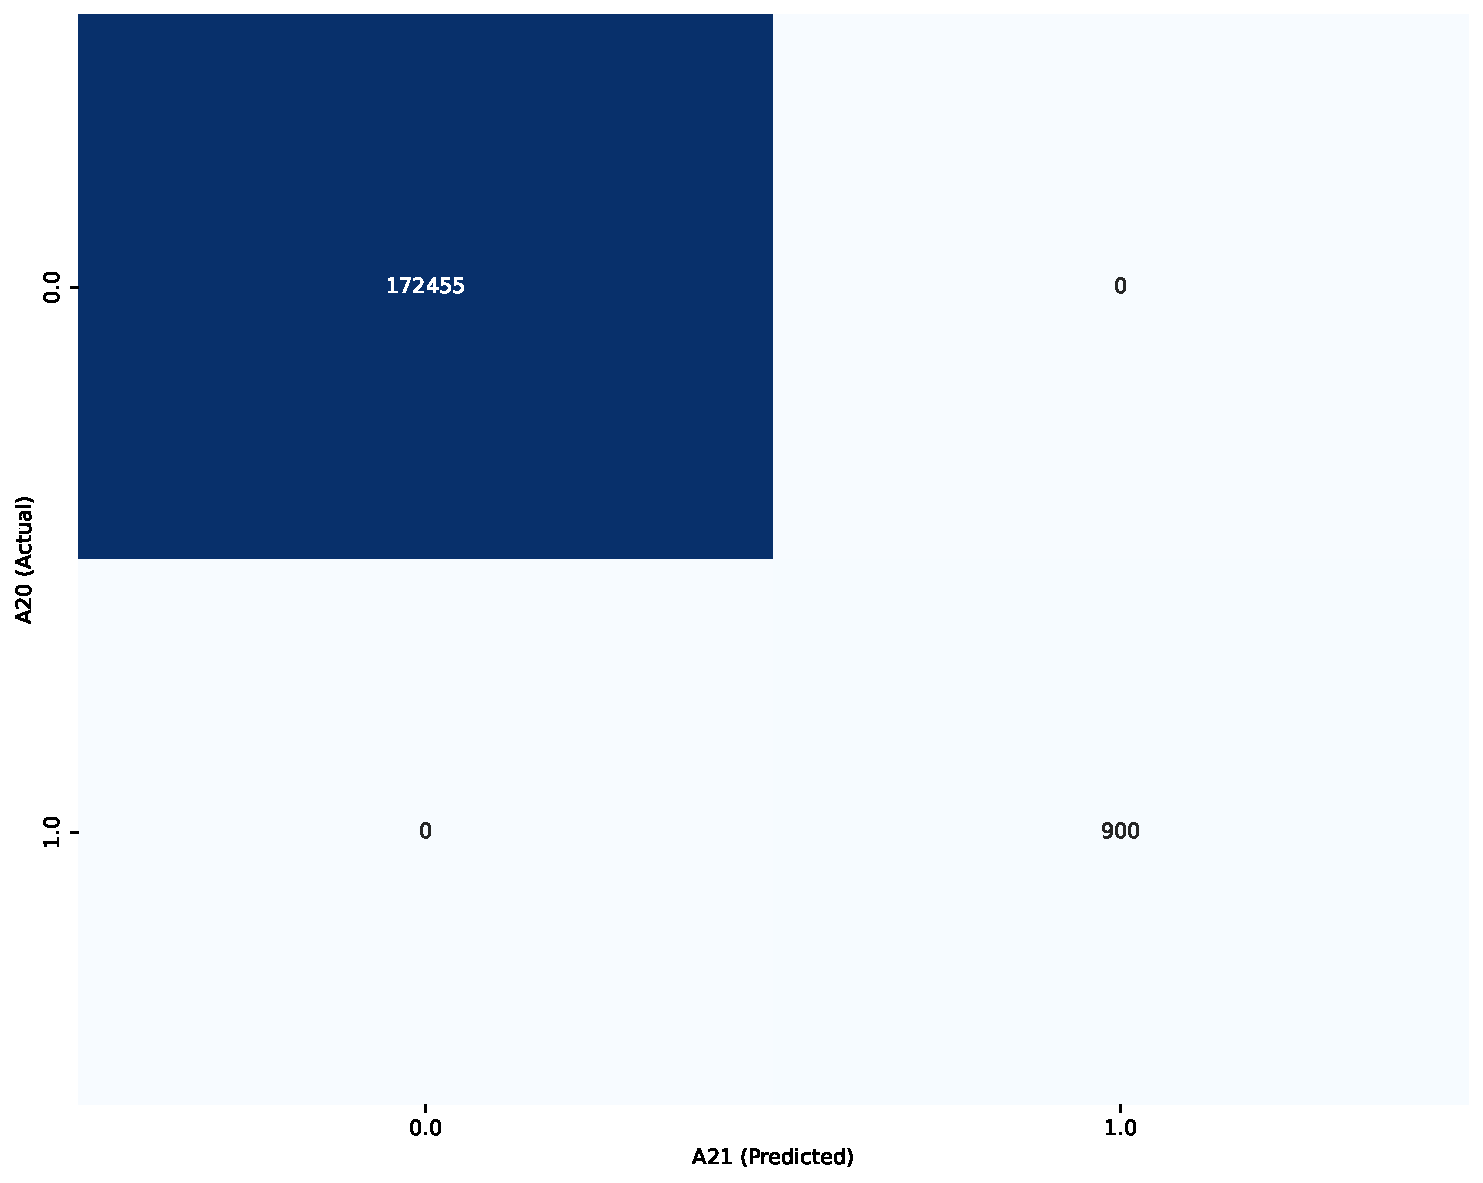
\includegraphics[width=\textwidth]{images/confusion_matrix_A20_A21.pdf}
		\caption{Confusion matrix of A20 vs A21}
		\label{fig:a20a21}
	\end{minipage}
\end{figure}


%\bibliographystyle{plainnat}
%\bibliography{references}


\end{document}
